\chapter{Machine Learning}
\label{chap:machine_learning}


\newpage

\section{Fundamentals}
The field of Machine Learning is concerned with algorithms which are able to `learn' from experience, this may be contrasted with algorithms which achieve some task with a set of static instructions \cite{DeepLearningBook}. The ability to learn allows these algorithms to solve problems which may be too complex for a collection of explicitly defined instructions. 
This chapter will give an overview of machine learning, and deep learning in particular, as pertinent to the field of high-energy physics. We begin with the fundamentals of machine learning, then move on to ensembling and decision trees, and finally neural networks and deep learning.  


\subsection{The Learning Process}

\subsubsection{Problem Formulation}
The data in a machine learning problem are often formulated in terms of a vector space $X = \mathds{R}^{n}$, where each dimension is an observable quantity referred to as a `feature' and a particular datum corresponds to a single feature vector $\vec{x} \in X$ \cite{elementsOfStatsLearning}. A dataset is represented as a set of feature vectors $\vec{x}_{i}$ and each can be considered to be drawn from some underlying probability distribution $F(\vec{x})$.
A machine learning algorithm can then be considered \cite{elementsOfStatsLearning} to consist of a model $f$, 
\begin{equation}
    f:(\vec{x},\vec{w})\rightarrow{Y}
\end{equation}
which is a function that maps from a feature vector $\vec{x}$ to an outcome $Y$ given a vector of parameters $\vec{w}$; a loss function $L$
\begin{equation}
    L:(f,\vec{x})\rightarrow{\mathds{R}}
\end{equation}
which measures performance given the model, a set of feature vectors and sometimes the desired outcome; 
and finally, an optimisation which tunes the parameters of the model with respect the loss to drive the learning process.


Learning is said to be occur when the model's performance at some class of tasks $T$ as measured by some performance measure $P$ improves given experience $E$ \cite{Learning} 
There are many classes of task which depend on the dataset and the desired outcome, but the two main classes of interest are classification and regression \cite{DeepLearningBook}:
\begin{itemize}[leftmargin=.5in,noitemsep]
    \item Classification tasks aim to predict a class given a feature vector, $f:\mathds{R}^{n}\rightarrow{}\{1,\dots,k\}$.
This is often an integer class label but can be a probability distribution over classes. An example of a classification problem from physics would be signal-background event discrimination where we attempt to classify events into background-like or signal-like classes.
    \item Regression tasks aim to predict a continuous value given the input features, $f:\mathds{R}^{n}\rightarrow\mathds{R}$. An example of a regression task in physics would be detector calibration where we attempt to predict the true value from the measured. 
\end{itemize}
In addition to these main classes of task there are others such as structured prediction that attempts to predict more complicated structures such as trees and lists, and many others. 


The experience that the model receives depends on the data that the model is exposed to during optimisation, and can be split into two broad categories \cite{DeepLearningBook}:
\begin{itemize}[leftmargin=.5in,noitemsep]
    \item Supervised machine learning algorithms experience target values $y$ as well as the input features $x$. They will experience multiple examples of feature vectors and attempt to reconstruct the correct value, with the loss calculated given the target. An example would be a classifier which is trained on simulated data where we know the true signal-background class label. 
    \item Unsupervised algorithms do not have access to target values and will attempt to infer information about the structure of the data such as clusters.
\end{itemize}



\subsubsection{Training and Evaluation}

The learning process is also referred to as `training' and has a different objective to a typical optimisation problem: rather than just finding the parameters which give the optimal loss over the training dataset, we require the model to find useful behaviours that generalise to new data \cite{DeepLearningBook}. 
To estimate the generalisation power of a model, we evaluate performance over another unseen dataset, the test set, which should be chosen such that it is representative of the distribution of the whole dataset.


During training most machine learning algorithms will use some form of gradient-based optimisation where one descends the gradient of $L$ with respect to $\vec{w}$ to find the minimum of $L$,
\begin{equation}
    \nabla_{\vec{w}}L = 0.
\end{equation}
The most conceptually simple approach is to evaluate this expression over the entire training set, however this is often impractical for large datasets which have a large population or high dimensionality. 

An alternative is to use stochastic gradient descent (SGD) \cite{DeepLearningBook}. With SGD we descend the gradient in steps where each step is performed by evaluating the gradient with small batches of training data (minibatches). 
The parameters are then updated as
\begin{equation}
    \vec{w} \rightarrow \vec{w} - \eta\nabla_{\vec{w}}L
\end{equation}
where $\eta$ is the learning rate, a parameter that controls the size of the steps at each parameter update. As we repeat this step the model parameters should ideally converge to a global optimum, but there are often local optima that the training can get settle into. 


\subsubsection{Example: linear regressor}
Now we have the ingredients of a machine learning algorithm, consider the simple example of a linear regressor. 

The dataset will consist of $n$-many points of single features, and the value to predict. These are distributed as a linear function with $\vec{w} = (-2,2)$ and a random noise component drawn from a Gaussian distribution

The task of linear regression is to predict the value $y$ given a collection of features. In this formulation we will consider a single feature $x$, and the algorithm will have access to the $y$ during training making this a supervised learning problem. 

The formula of the model is
\begin{equation}
    \hat{y} = w_{1} + w_{2}x,
\end{equation}
and the term linear refers to the model parameters, powers of $x$ are considered features. 
The loss will be the mean squared error,
\begin{equation}
    L = \frac{1}{n}\sum_{i=1}^{n}(\hat{y}_{i}-y_{i})^{2},
\end{equation} 
and a single SGD step will be 
\begin{equation}
    \begin{pmatrix}
        w_{1} \\
        w_{2}
    \end{pmatrix} \rightarrow
    \begin{pmatrix}
        w_{1} \\
        w_{2}
    \end{pmatrix} - \eta
    \frac{1}{m}\sum_{i=0}^{m}
    \begin{pmatrix}
        2(w_{1}+w_{2}x_{i} - y_{i})\\
        2x_{i}(w_{1}+w_{2}x_{i} - y_{i}),
    \end{pmatrix}
\end{equation}
where $m$ is the minibatch size.

The training is performed for $500$ minibatches with a learning rate of $0.0001$ and parameters initialised to $1$. The training process and final outcome of this algorithm are shown in Figure \ref{fig:machine_learning:lin_example}.

\begin{figure}[h!]
    \begin{center}
        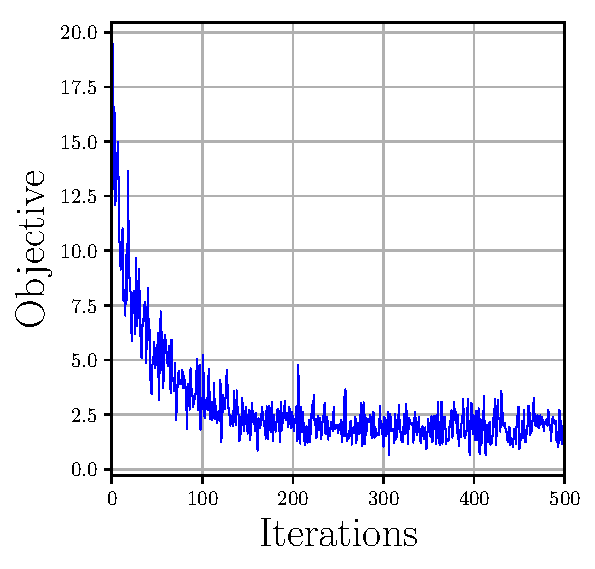
\includegraphics[width=0.32\textwidth]{figures/machine_learning/loss_history.pdf}
        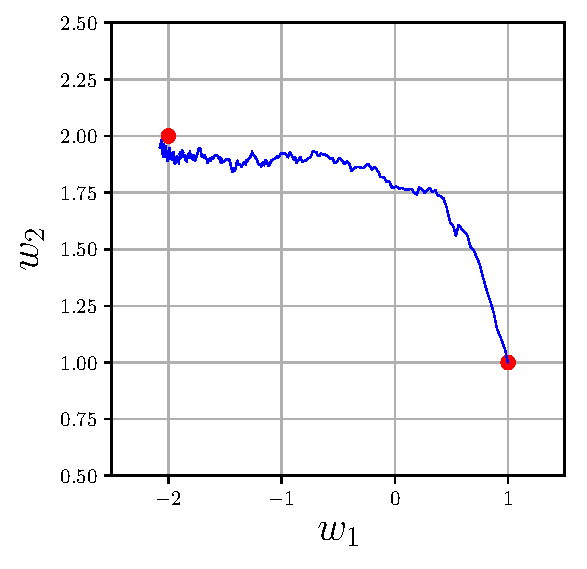
\includegraphics[width=0.32\textwidth]{figures/machine_learning/w1_w2_history.pdf}
        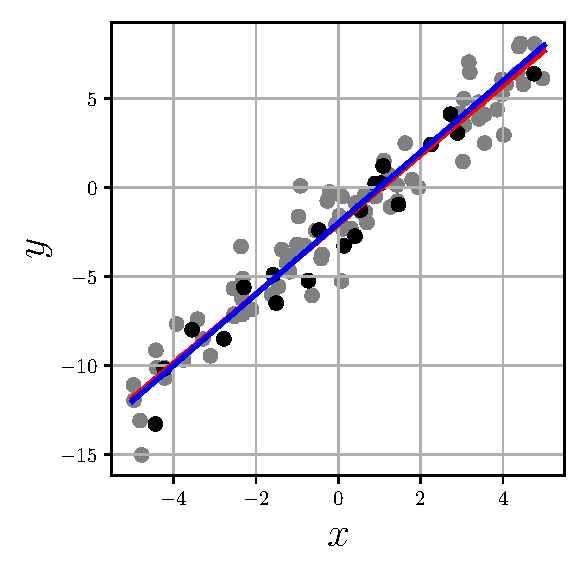
\includegraphics[width=0.32\textwidth]{figures/machine_learning/data_and_results.pdf}
    \end{center}
    \caption{Training a linear regressor. Loss history over training (left), the trajectory of the model parameters in parameter space during training (centre), and the final result with the result in read and the true value in blue, an example minibatch is shown by the black points (right).}
        \label{fig:machine_learning:lin_example}
\end{figure}








\subsection{Model Capacity and Generalisation}

The space of functions which a model can draw upon to describe observed data is referred to as the model's hypothesis space.
Taking the example of a linear regressor, the hypothesis space can be expanded by using higher-order polynomials
\begin{equation}
    \hat{y} = \sum_{i=0}^{N}w_{i}x^{i}.
\end{equation}
When we increase or decrease the size of this space we are increasing and decreasing the model's descriptive power, known as its `capacity' \cite{DeepLearningBook}, and if it is inappropriately large or small the model can experience problems with generalisation.
Specifically, over or under-capacity can lead to generalisation error from two sources which often need to be traded against each other: bias and variance. Bias is the error that comes from the model approximating the underlying function, variance is how much the trained model estimate will change if we change the training dataset \cite{DeepLearningBook}. 

If the capacity is too small this leads to `underfitting' where the model does not have enough descriptive power to fit the data and we get generalisation error due to bias. If there is too much capacity the model will find a function fit to the training set arbitrarily well and have large variance, this will cause another sort of generalisation error called `overfitting'. Examples of how inappropriate capacity can lead to a failure to generalisation error are shown in Figure \ref{fig:machine_learning:overfitting} where a linear regressor is trained with different order polynomials. 
\begin{figure}[h!]
        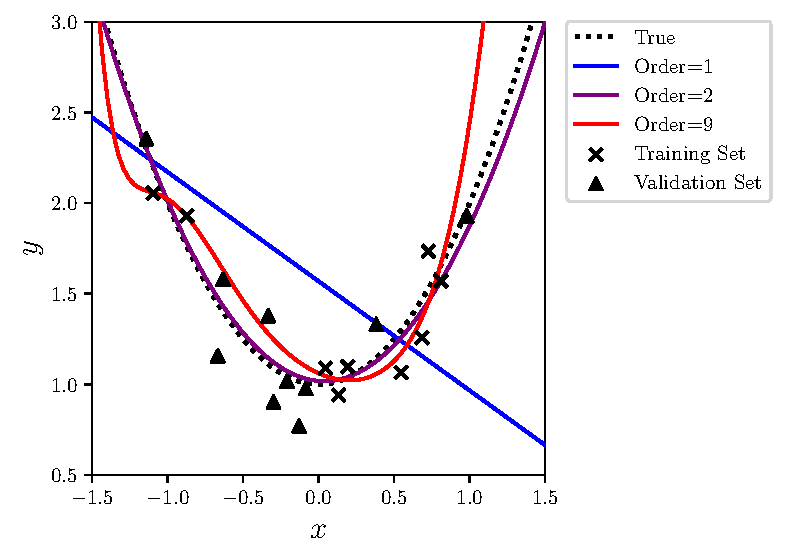
\includegraphics[width=0.6\textwidth]{figures/machine_learning/capacity.pdf}
    \caption{Linear regressors with different order polynomials fitted to the same data. }
        \label{fig:machine_learning:overfitting}
\end{figure}
In this example we note that the high-capacity model has been fitted to noise and fails to generalise to unseen data. 

An alternative and more general approach to controlling model capacity is to penalise parts of the hypothesis space rather than remove them, which could be considered infinite penalisation. This way, if we have two functions which perform equally well, we can express some sort of preference for which one to choose by adding a term to the loss. This penalty term is called a `regulariser' term \cite{DeepLearningBook} and has the form
\begin{equation}
    \lambda\Omega(\vec{w}),
\end{equation}
where $\lambda$ is a value which scales the strength of the regulariser's effect. The variable $\lambda$ is an example of a `hyperparameter' which is defined as any unlearned parameter of a machine learning algorithm. Furthermore, adding regulariser terms to the loss is an example of regularisation, a broad class of techniques which aim to improve an algorithm's generalisation error. 


Two common forms of regularisation are penalty terms based on the squared-$L^{2}$ and $L^{1}$ norm of the model's weight vector
\begin{equation}
    \begin{split}
        \lambda||\vec{w}||^{2}_{2} =& \lambda\sum_{i=0}^{n}w_{i}^{2} \\
        \lambda||\vec{w}||_{1} =& \lambda\sum_{i=0}^{n}|w_{i}|. \\
    \end{split}
\end{equation}
These two regularisers have a different effect on the model parameters: $L^{2}$ regularisation expresses a preference for using each parameter a small amount, $L^{1}$ regularisation will prefer sparsity where a few parameters are large, and the rest close to zero. 
A comparison of a range of values for both regularisers applied to a linear regressor with a $9^{\mathrm{th}}$-degree polynomial is shown in Figure \ref{fig:machine_learning:reg_example}. 
\begin{figure}[h!]
    \begin{center}
        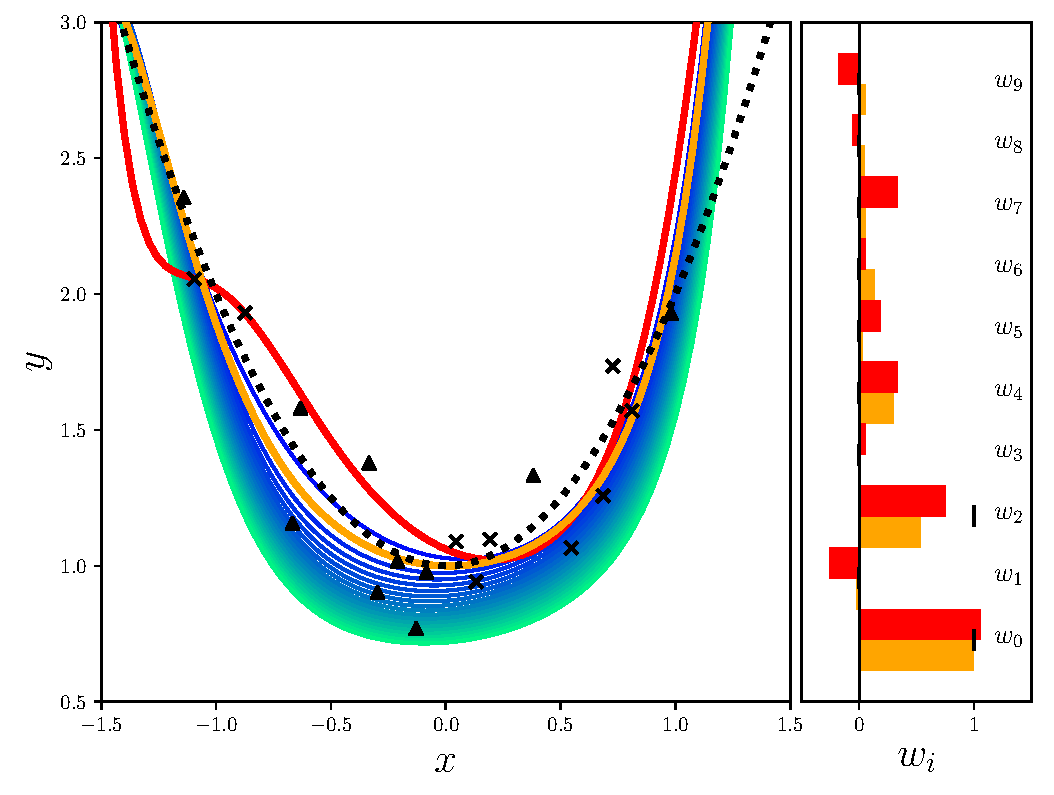
\includegraphics[width=0.49\textwidth]{figures/machine_learning/L2_reg_plot.pdf}
        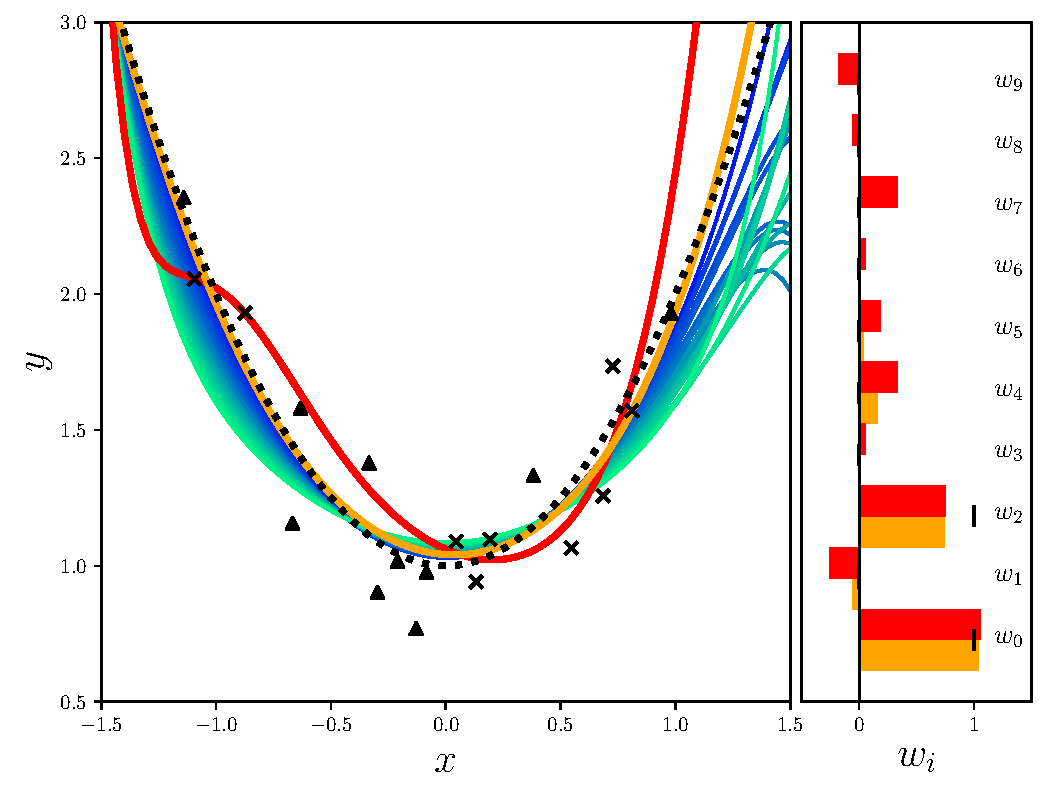
\includegraphics[width=0.49\textwidth]{figures/machine_learning/L1_reg_plot.pdf}
    \end{center}
    \caption{Fits for different regularisation strengths with $L^{2}$ (left) and $L^{1}$ (right) regularisation data drawn from a uniformly sample of $y=1+x^{2}$ plus noise. The red curve is the unregularised fit, the orange curve is the result with the lowest loss with respect to the validation set (triangles). The bar charts show the parameter values of the overfitted result and optimal regularised result.} 
        \label{fig:machine_learning:reg_example}
\end{figure}
These models have been evaluated for generalisation error on another unseen dataset: the `validation' set. The reason to use this rather than the test set is that when we choose a hyperparameter value we are essentially doing another fit to data. If we do this on the test set we may fit to unrepresentative patterns in the test data and overfit again. Evaluation on the test set is then no longer a good measurement of generalisation. 








\subsection{Ensembles}

It is sometimes useful to train multiple models (base learners) and combine them in some way, for example by some weighted sum of their outputs, chaining them together, or some other approach. This technique is called ensembling, and one of the most popular machine learning algorithms in particle physics is an example of this: boosted decision trees (BDTs) \cite{MiniBooneBDT}. This subsection will give only a narrow overview of this area as relevant to the CMS Higgs diphoton analysis: we will focus on a single ensembling method, gradient boosting, and a single base learner the decision tree.


\subsubsection{Decision Trees}
Decision trees \cite{DecisionTrees} are binary tree structures which recursively partition the feature space into non-overlapping regions. Each node of the tree corresponds to a region, each additional child node corresponds to further splits into subregions. One eventually reaches a node with no child, this last node is a leaf of the tree and assigns a value to the corresponding region.  
Decision trees are trained by calculating a collection of possible splits and then choosing one which optimises a measure of purity in classification case, or a loss function such as mean-squared error in the regression case. This process is usually stopped once the leaf nodes have reached some optimal value, or a maximum depth has been reached. 
Decision trees are also regularised by pruning which removes branches that use unimportant features. 

Decision trees have advantages such as their simplicity, interpretability, and their ability to handle different types of data. However, they also have various disadvantages such as their cuts being aligned with the dimensions of the feature space, so diagonal decision boundaries need to be constructed out of many orthogonal cuts, their tendency to get stuck in local minima, and their training variance which leads to overfitting. These disadvantages can be mitigated by using decision trees as base learners in an ensemble which produces an algorithm stronger than its constituent parts. 

\subsubsection{Gradient Boosting of Decision Trees}
Generally, boosting algorithms \cite{Boosting} construct a strong learner from base learners by iteratively training base learners which compensate for earlier weakness in some way. Each base learner is then added together in a weighted fashion to produce the final ensemble.
Gradient boosting \cite{GradientBoosting} is a particular boosting algorithm which uses fitting to the errors of prior base learners and gradient descent. Gradient boosting assumes that at each iteration $n$, $1<n\leq{N}$ there is a base model $f_{n}(\vec{x})$ which can be improved by addition of another estimator (in our case another decision tree) $h(\vec{x})$
\begin{equation}
    f_{n+1}(\vec{x}) = f_{n}(\vec{x}) + h(\vec{x}).
\end{equation}
If $h(\vec{x})$ perfectly corrects $f_{n}(\vec{x})$ this implies that,
\begin{equation}
    \begin{split}
        f_{n+1}(\vec{x}) &= f_{n}(\vec{x}) + h(\vec{x}) = y \\
        h(\vec{x}) &= y - f_{n}(\vec{x}) \\
    \end{split}
\end{equation}
where $y - f_{n}(\vec{x})$ is referred to as the `residual'. A key insight was that this process is analogous to gradient descent as the residuals are the negative gradients with respect to $F(\vec{x})$ of the squared error loss function
\begin{equation}
    \frac{1}{2}(y-F(\vec{x}))^{2}.
\end{equation}
This can then be generalised to other differentiable loss functions. 

When the base learners are decision trees the process is as follows: at each iteration $n$ we train a DT on the residual 
\begin{equation}
    h_{n}(\vec{x}) = \sum_{j=1}^{J_{n}}b_{jn}\mathbf{1}_{R_{jn}}(\vec{x})
\end{equation}
where $J_n$ is the number of regions of $h_{n}$, $R_{1n},\dots,R_{J_{n}n}$ are the regions themselves, $b_{jn}$ is the value predicted in region $R_{jn}$, and $\mathbf{1}_{R_{jn}}$ returns $1$ for $\vec{x}$ in region $R_{jn}$ and zero otherwise. 
The output of this tree is multiplied by a value $\gamma_{n}$ which minimises the loss chosen by line search,
\begin{equation}
    \gamma_{n} = \mathrm{argmin}_{\gamma}\sum_{i=1}^{m}L(y_{i},f_{n-1}(\vec{x})+\gamma{}h_{n}(\vec{x}_{i})),
\end{equation}
and then the ensemble is added to as
\begin{equation}
    f_{n}(\vec{x}) = f_{n-1}(\vec{x}) +\eta\gamma_{n}h_{n}(\vec{x}_{i}).
\end{equation}
where $\eta$ is a learning rate parameter and controls steps size just like in normal gradient descent. 




\subsection{Algorithm Design and Optimisation}

% No free lunch theorem
The No Free Lunch theorem of machine learning \cite{NoFreeLunch} states that, averaged over all possible data-generating distributions, every classification algorithm has the same error rate when classifying previously unobserved points.
This result essentially means that no machine learning algorithm is universally superior, but it does not mean that they are all equally-powerful for a particular task. 
The theorem only holds averaged over all distributions, and some algorithms will indeed perform better given specific focus: we must make assumptions given prior knowledge and build our algorithms accordingly.
This will inform how we choose the model, how we measure performance, and how we optimise the hyperparameters. 


% Curse of dimensionality
A particularly important phenomenon is the `curse of dimensionality' \cite{elementsOfStatsLearning} where machine learning algorithms can under-perform given a dataset with a large number of features (high-dimensionality).
For such a dataset the number of possible configurations of the features are far larger than the size of the training set. 
This can also be formulated in terms of coverage of a hypervolume (Figure \ref{fig:machine_learning:curse_of_dimensionality}): if one considers a unit cube of dimension $D$, the portion of the sides required to cover a given volume increases rapidly with $D$.
This issue is a primary motivator for the development of deep learning, and is also something that needs to be considered during hyperparameter optimisation. 
\begin{figure}[h!]
    \begin{center}
        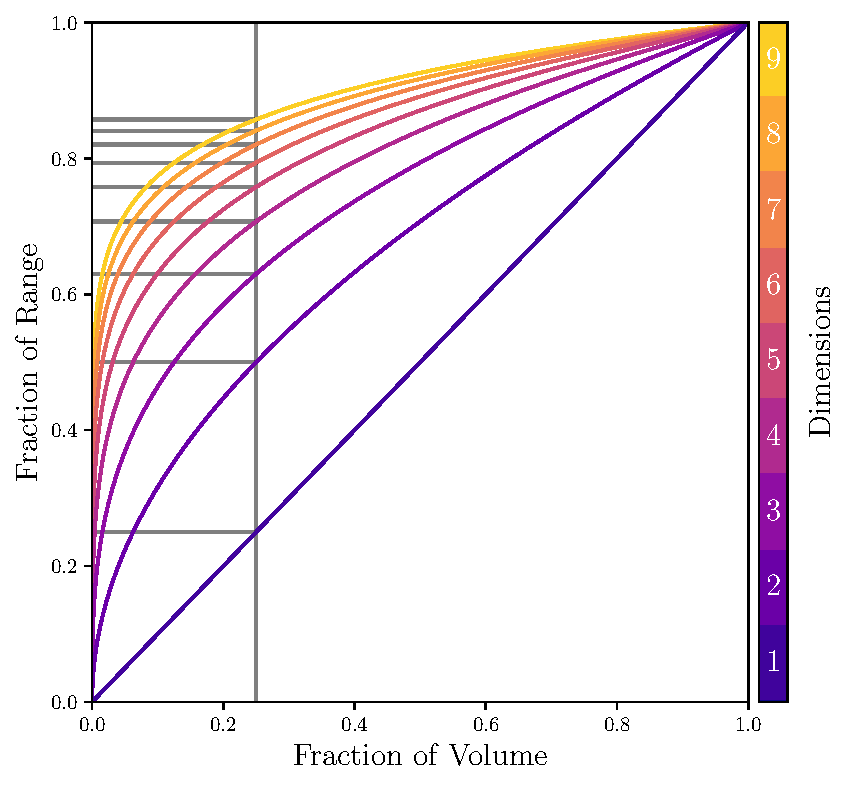
\includegraphics[width=0.4\textwidth]{figures/machine_learning/curse_of_dimensionality.pdf}
    \end{center}
    \caption{Range of the side length to cover a fraction of the volume of a unit cube in up to nine dimensions. The grey lines show the fraction required to cover 25\% of the volume.}
        \label{fig:machine_learning:curse_of_dimensionality}
\end{figure}


% What's to be designed? Model, objective, task, experience and constraints
Choice of model, and input features, will depend on a number of practical constraints such as time and computational resources, but also constraints that avoid biases particular to physics analyses. 
In training a classifier to separate Higgs boson signals on simulation we do not want the algorithm to reconstruct the mass and bias itself to the simulation value. This can happen if the algorithm is given this value explicitly or if it is capable to reconstructing it from the other features.  
Furthermore one must use assumptions from prior knowledge of dataset size, dimensionality and other properties such as linear separability and class balance to choose the model. One can then evaluate candidate algorithms using appropriate performance measures. 


% Hyperparameters
Once the model is chosen hyperparameters can be selected with a variety of optimisation approaches. However, because the underlying function which maps from hyperparameters to performance values is unknown we cannot use gradient-based methods. Here we use derivative-free optimisation methods, two of which will be presented here and used later in this thesis: grid search and Bayesian optimisation.

% Optimisation with grid search
Grid search is a simple method which simply samples a set of evenly-spaced values over a given region of the hyperparameter space. 
This method can be used when there are fewer hyperparameters to optimise and the time cost of sampling each point is not too great. 
As the number of hyperparameters goes up, dimensionality increases and the sampling becomes extremely sparse as each point represents a smaller portion of the space.

% Optimisation with Bayesian Optimisation
Bayesian optimisation \cite{BayesOpt} is part of a class of optimisation algorithms that use previous observations of the performance to determine the next point to sample. 
The method consists of two main steps:
\begin{enumerate}[leftmargin=.5in,noitemsep]
    \item using evaluated points in the hyperparameter space calculate a posterior expectation of the performance as a function of the hyperparameters
    \item evaluate the performance at a new point which maximises an 'acquisition function', a function which scores how optimal a point in the hyperparameter space is to evaluate. 
\end{enumerate}
Bayesian optimisation makes efficient use of sampling and is more appropriate when evaluating a single point in the hyperparameter space is expensive. The difficulty of the optimisation will still increase rapidly with the dimensionality so one should consider, where possible, the optimisation as a set of orthogonal problems.  
These two methods can be combined where an initial grid search is performed, and the set of evaluated points are used in the first iteration of the Bayesian optimisation. 
This step is called a `warm start'. 

Often we do not know the form of the data-generating distribution a priori. Therefore a good approach to choosing and tuning a model is to have as much capacity as design constraints allow and then restrict this capacity with regularisation using an optimisation over the validation set as described earlier.

\section{Deep Learning}

Deep learning offers a powerful approach to supervised learning problems based on artificial neural networks (ANNs), especially when there are large quantity of input features. 
The name of the field refers to the depth of the ANNs, as depth increases they can model ever-more complex functions of the input data. 
This section will give a description of ANNs, how they are trained and regularised, the challenges that come with increasing network depth, and finally convolutional neural networks and specifically dense convolutional neural networks.  

\subsection{Artificial Neural Networks}

\subsubsection{The Single Neuron}
Artificial neurons receive a weighted collection of input signals and then `fire' depending on their sum \cite{CS231n}. Mathematically, they consists of an input feature vector $x_{i}$, a weight vector $w_{i}$, a bias $b$ and a nonlinear activation function $f$ which produces an output $o$ via the following computation,
\begin{equation}
    o = f(w_{i}x_{i} + b).
\end{equation}
A schematic of an artificial neuron is shown in Figure \ref{fig:machine_learning:neuron_and_activation} along with two commonly used activation functions. 
\begin{figure}[h!]
    \begin{center}
        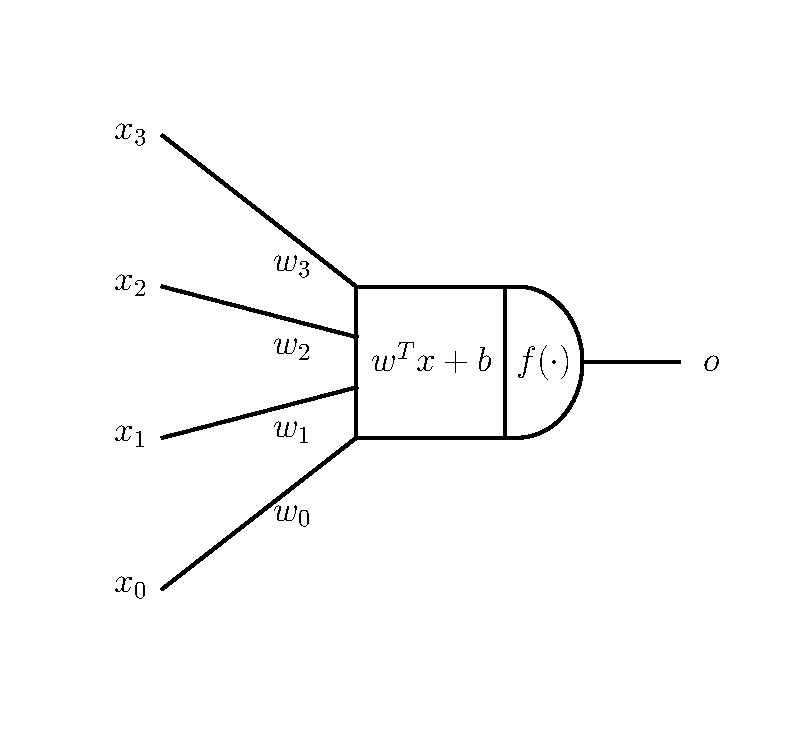
\includegraphics[width=0.4\textwidth]{figures/machine_learning/neuron.pdf}
        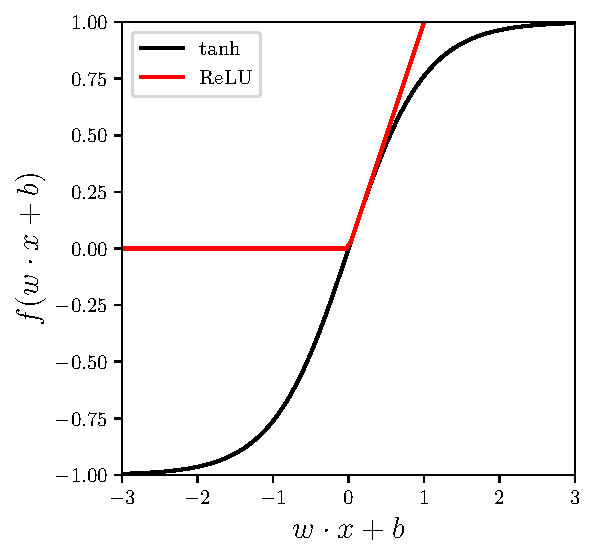
\includegraphics[width=0.4\textwidth]{figures/machine_learning/activation_functions.pdf}
    \end{center}
    \caption{Schematic of an artificial neuron(left) and two activation functions (right).}
        \label{fig:machine_learning:neuron_and_activation}
\end{figure}
The weight vector and the bias constitute the learnable parameters of this model. 
With the correct loss and activation this structure is equivalent to a linear classifier, so we can consider each neuron to be attempting to place an optimal linear decision boundary in the space of its input features. 
If the data are linearly-separable this will be achievable, but if they are not this simple classifier will struggle. 
To help the neuron one could consider a function $\phi(x_{i})$ on the feature space to produce transformed feature vectors in which the data are now linearly separable \cite{DeepLearningBook}. 
One could construct this function explicitly, or it could be learned from data. 



\subsubsection{Feedforward Neural Networks}
ANNs come in many different architectures, but the ones we will consider here will be exclusively feedforward networks. 
These networks are constructed from layers of neurons where each layer feeds into the ones after it, starting with the input layer, then often multiple hidden layers, with the final output layer giving the prediction. 
The most common layer type used is the `fully-connected' layer where each neuron in layer $l$ is connected to every neuron in layer $l+1$. 

A classic feedforward architecture is the multi-layer perceptron (MLP) which consists of a series of fully-connected layers. Often the outputs $\vec{o}$ of these networks are fed through the `softmax' function which maps these outputs to a vector of probabilities that sum to one,
\begin{equation}
    \sigma(\vec{o})_{i} = \frac{e^{o_{i}}}{\sum_{k=1}^{N}e^{o_{k}}},
\end{equation}
where $N$ is the number of outputs. 

When we connect multiple layers together we are constructing a model which is capable of performing a chain of feature space transformations $\phi(x_{i})$ where each layer produces features for the one that follows it, and the final layer can place a linear decision boundary on this transformed feature space \cite{DeepLearningBook}. 
The effect of composing layers together can be seen by comparing a model with no hidden layers versus a model with a single hidden layer on data which is not linearly separable (Figure \ref{fig:machine_learning:mlp_example}).

\begin{figure}[h!]
    \begin{center}
        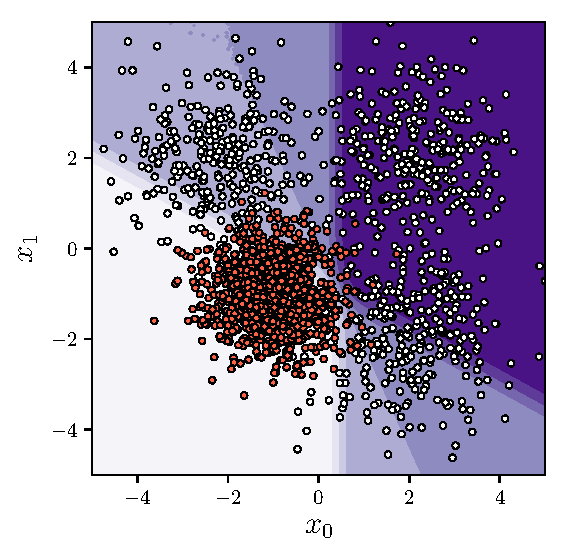
\includegraphics[width=0.45\textwidth]{figures/machine_learning/decision_bound_tanh_depth_1.pdf}
        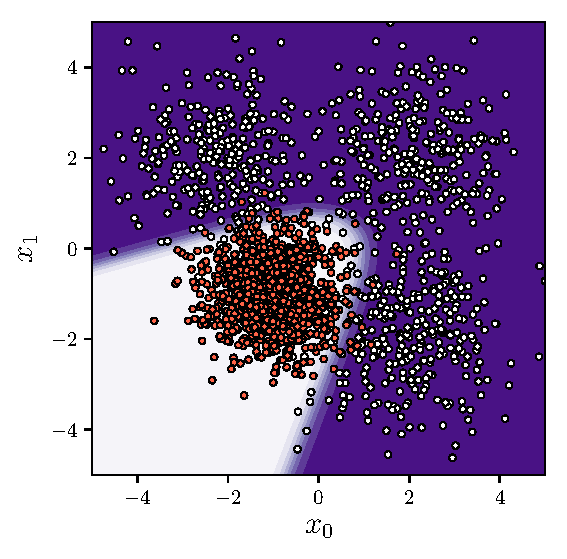
\includegraphics[width=0.45\textwidth]{figures/machine_learning/decision_bound_tanh_depth_2.pdf}
    \end{center}
    \caption{Decision boundaries for a two-input ($x_{0}$, $x_{1}$), two-class neural network classifier with no hidden layer (left) and one hidden layer (right). The output of the networks are mapped to probabilities with the softmax function and are shown by the background contour plot. }
        \label{fig:machine_learning:mlp_example}
\end{figure}
With increasing depth neural networks are able to construct ever-more complex functions of their input. 
Mathematically, this corresponds to repeated matrix multiplication of a feature vectors plus biases interleaved with non-linear activation functions,
\begin{equation}
    o_{k} = f_{n}(f_{n-1}(\dots{}(f_{1}(w^{1}_{ij}x_{i} + b^{1})))).
\end{equation}



\subsubsection{Training Neural Networks}

%Loss 
ANN classifiers may use a variety of different loss functions. 
Let $o_{j}$ indicate the $j^{\mathrm{th}}$ element of the output class vector of the neural network and $y_{i}$ indicate the true class label of datapoint $i$. 
Two popular choices of loss function \cite{CS231n} are the hinge loss and cross entropy loss with softmax function.
The hinge loss has the form
\begin{equation}
    L_{i} = \sum_{j\neq{}y_{i}}\mathrm{max}(0,o_{j}-o_{y_{i}} + 1)
\end{equation}
and is a `maximum margin' loss which attempts to strongly penalise misclassified examples. 
The cross entropy loss has the form
\begin{equation}
    L_{i} = -\mathrm{log}\left(
        \frac{e^{f_{y_{i}}}}
        {\sum_{j}e^{o_{j}}}\right)
\end{equation}
and is used in conjunction with a softmax function. This loss can be interpreted as minimising the negative log likelihood of the correct class.
Each of these will cause the network to behave in a different way: the hinge loss will in effect prioritise accurate classification at the cost of modelling probability whereas the cross entropy will model $p(y|x_{i})$ with less priority on accuracy \cite{CS231n}.

%Backprop
Once the loss has been defined, neural networks are trained via gradient descent with an algorithm called back-propagation \cite{Backprop}. A single iteration works as follows:
\begin{enumerate}[leftmargin=.5in,noitemsep]
    \item Forward pass: inputs are repeatedly repeatedly transformed from the first layer to the last with product sums dependent on $w_{ij}^{k}$ and then by the activation functions. The final output $\hat{y}$, the input to each activation, and the output from each activation are stored for the next step. 
    \item Backward pass: this works like the forward pass but from the output layer backwards to the input calculating $\partial{L}/\partial{w_{ij}^{k}}$ as it goes. The ``inputs'' are the output layer's loss terms and these are repeatedly transformed by product sums with the weights $w_{ij}^{k}$ and then by the derivatives of the activation functions.  
    \item Weight update: after the backward pass we now have the gradients required to update the weights by typical gradient descent.
\end{enumerate}


\subsubsection{Regularising Neural Networks}
Just like other machine learning models neural networks will overfit when they have too much capacity and regularisation is crucial. The $L^{1}$ and squared-$L^{2}$ regularisers are commonly used and $L^{2}$ is often preferred \cite{CS231n}. Another regularisation method is max-norm clipping \cite{CS231n} which restricts the norm of the gradient vectors during weight update and stops them from getting above a certain size whilst preserving their direction in parameter space. Finally, a highly-effective and complimentary method is `dropout' \cite{Dropout} (Figure \ref{fig:machine_learning:dropout})  where neurons are switched off at random. This aids model generalisation by stopping the network from over-using neurons and also acts as an effective ensembling where many random subnetworks are trained then combined together at inference time.  
\begin{figure}[h!]
    \begin{center}
        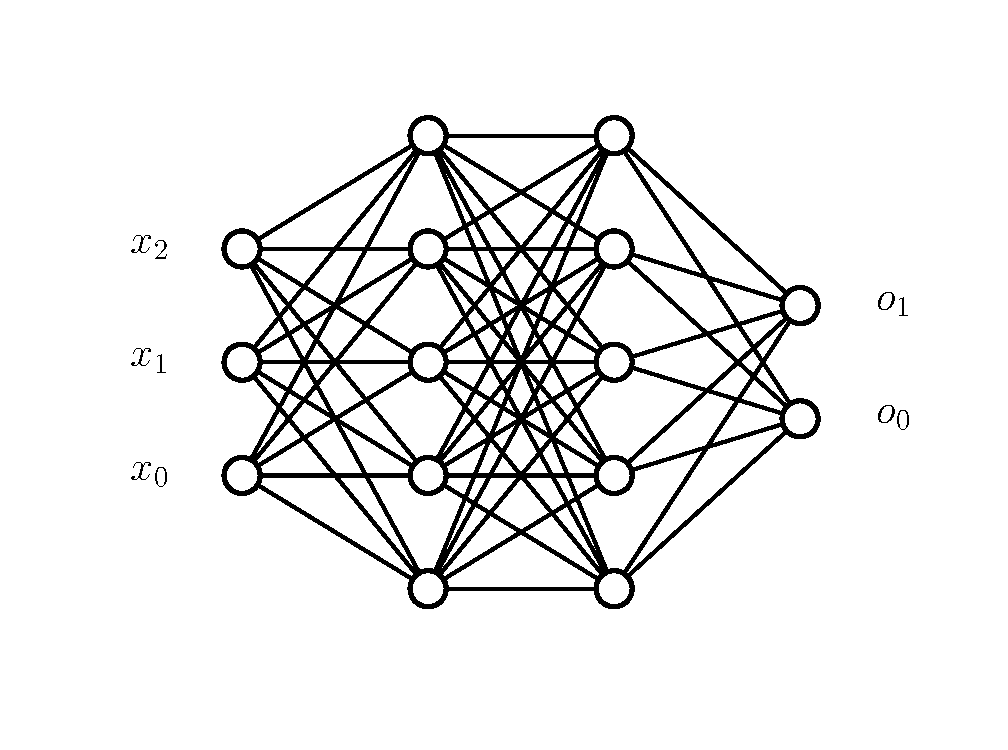
\includegraphics[width=0.45\textwidth]{figures/machine_learning/no_dropout.pdf}
        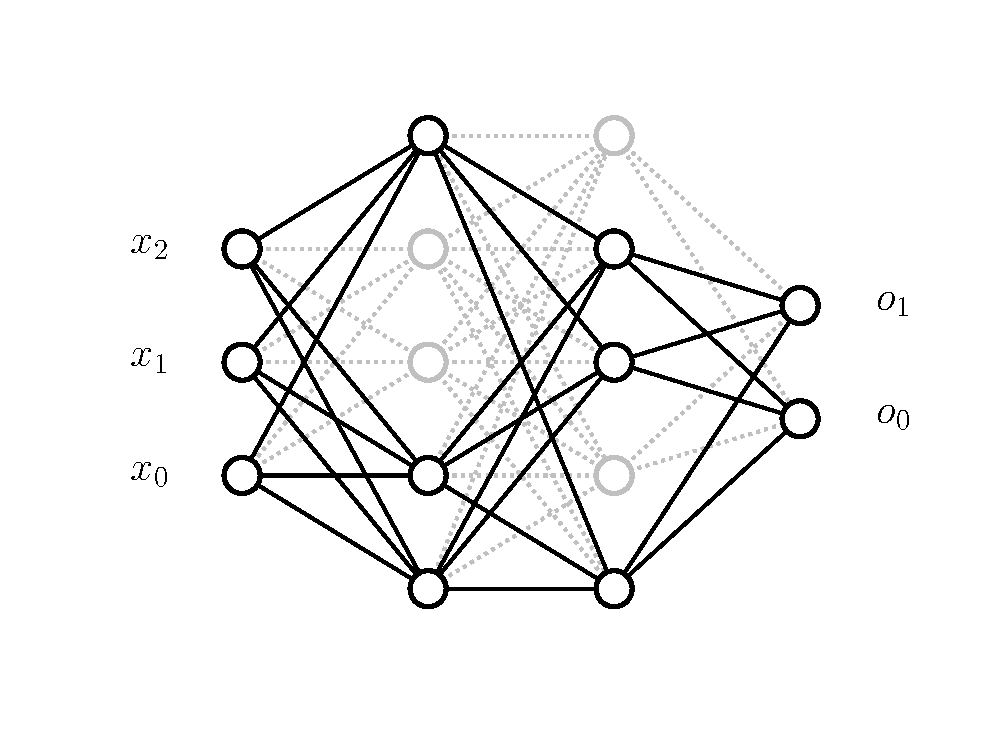
\includegraphics[width=0.45\textwidth]{figures/machine_learning/dropout.pdf}
    \end{center}
    \caption{Left: a multi-layer perceptron with no dropout. Right: the same network with dropout with dropped neurons are shown greyed out.}
        \label{fig:machine_learning:dropout}
\end{figure}

Additionally, although they are not strictly regularisations, data preprocessing and augmentation can greatly help with model generalisation. Augmentation is when we apply random transformations to the input features such as random rotations and reflections of an image. Standardisation is when each of the features are mean-subtracted and divided by their standard deviation so that each feature has zero mean and unit variance. This helps greatly with training time and convergence. 


\subsubsection{Network Depth and its Problems}
As one simply increases the depth of a neural network the performance does not always increase. Depth brings with it a collection of problems each of which have their solutions and therefore an impact on network design. 

A major problem that occurs with deep ANNs which use sigmoidal activation functions is the vanishing/exploding gradient problem \cite{VanishingGradient}. During training these functions can have gradients in the range $[0,1]$ which are multiplied $n$-many times given how many layers from the output layer the backward pass is. This causes the gradients to become small, the weight updates in turn become small, and the training slows down heavily or stops altogether. If the gradients are greater than one the opposite problem can happen where the gradient becomes very large, this will cause inputs to neurons to become large and push the activation functions into the saturation region where the gradient is again small. 
This can be mitigated by using a non-sigmoidal activation such as ReLU, and choosing the correct weight initialisation (drawn from a Gaussian with $\mu=0$ and $\sigma=\sqrt{2/n}$ where $n$ is the number of elements in $w_{ij}^{k}$ \cite{HeEtAl}). 

Another problem is internal covariate shift \cite{BatchNorm}: because the input to each layer depends on all the ones before it, small changes can be amplified and cause the distributions in later layers to shift. This makes learning in later layers harder. 
To solve this issue we introduce `batch normalisation' layers \cite{BatchNorm}. These layers normalise the input into each layer on a per-minibatch basis during training and also have a learnable scale and shift
\begin{equation}
    \gamma\frac{x-\mu}{\sigma} - \beta.
\end{equation}
During inference the population statistics of the layer inputs are used, this must be calculated from the training set during the training process. These layers also help with the vanishing gradient problem. 

Finally, even with the above measures in place the accuracy of a deep network can saturate as depth increases and then drop. This is not caused by overfitting but is actually caused by the network's failure to reproduce identity transformations leading to the degradation of information as it passes to deeper layers \cite{ResNet}. This has been solved by using different sorts of bypass connections where outputs from earlier layers are directly connected to later ones to facilitate the flow of information. This was the key insight that drove the development of the ResNet architecture \cite{ResNet}, and the dense convolutional network architecture used in this thesis.  


\subsection{Convolutional Neural Networks}
Convolutional Neural Networks (CNNs) are aimed at image processing tasks and have achieved remarkable levels of performance. 
These networks make certain assumptions about their inputs which allow them to avoid the problems of an ordinary MLP if it were to be applied to an image processing problem. 
MLPs will struggle with with these tasks as they are high-dimensional in their input, and the fully-connected layers of MLPs do not scale well with larger input spaces. 
For example, if the input image is a $100\times{}100\times{}3$ RGB image each neuron in the next fully-connected layer would receive $30000$ inputs, leading to a very large number of parameters in even a shallow network. 
A network with such a large number of parameters will be difficult to train and will suffer from overfitting.

CNNs are feedforward-type ANNs constructed from successive 3D volumes of neurons which use local connectivity and weight sharing to avoid the issues with MLPs in this area \cite{CS231n}. Specifically, CNNs introduce two new layer types: convolution layers and pooling layers.

\subsubsection{Convolution Layers}
Convolution layers learn to find local features in the image which are then transformed into ever-more abstract and complex features in deeper layers. 
These features are not engineered but learned and allow the CNN to construct collections of useful features with minimal human involvement.


A convolutional layer receives a 3D volume of input values and will map this to another 3D volume of output values which will not necessarily have the same size. 
The layer itself consists of a 3D volume of neurons each of which views a small portion of the input width and height (its field of view) and usually the full extent of the depth. 
Each of these neurons will share the same weight values as its neighbours at the same depth and each will look for the same feature in a different place. 
These can be considered to be like learned filters that scan across the image and map a patch of input to a scalar value. The way they are spaced (or alternatively how the filter moves) is referred to as the stride. 
The output volume of neuron activations can be considered to be $n$-many transformed versions of the input where $n$ is the number of filters. This output is referred to as a feature map. 
\begin{figure}[h!]
    \begin{center}
        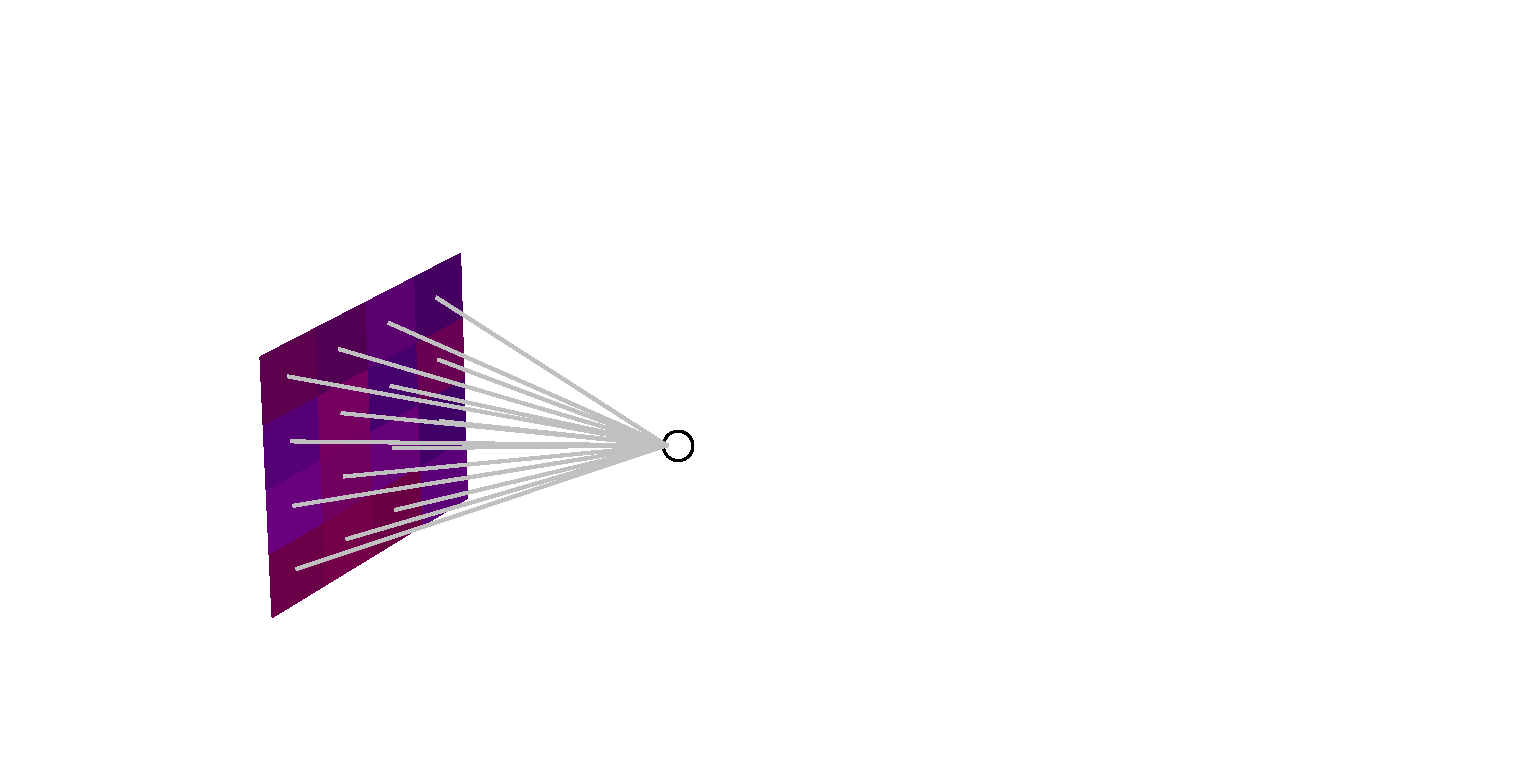
\includegraphics[width=0.32\textwidth]{figures/machine_learning/convolution_neuron.pdf}
        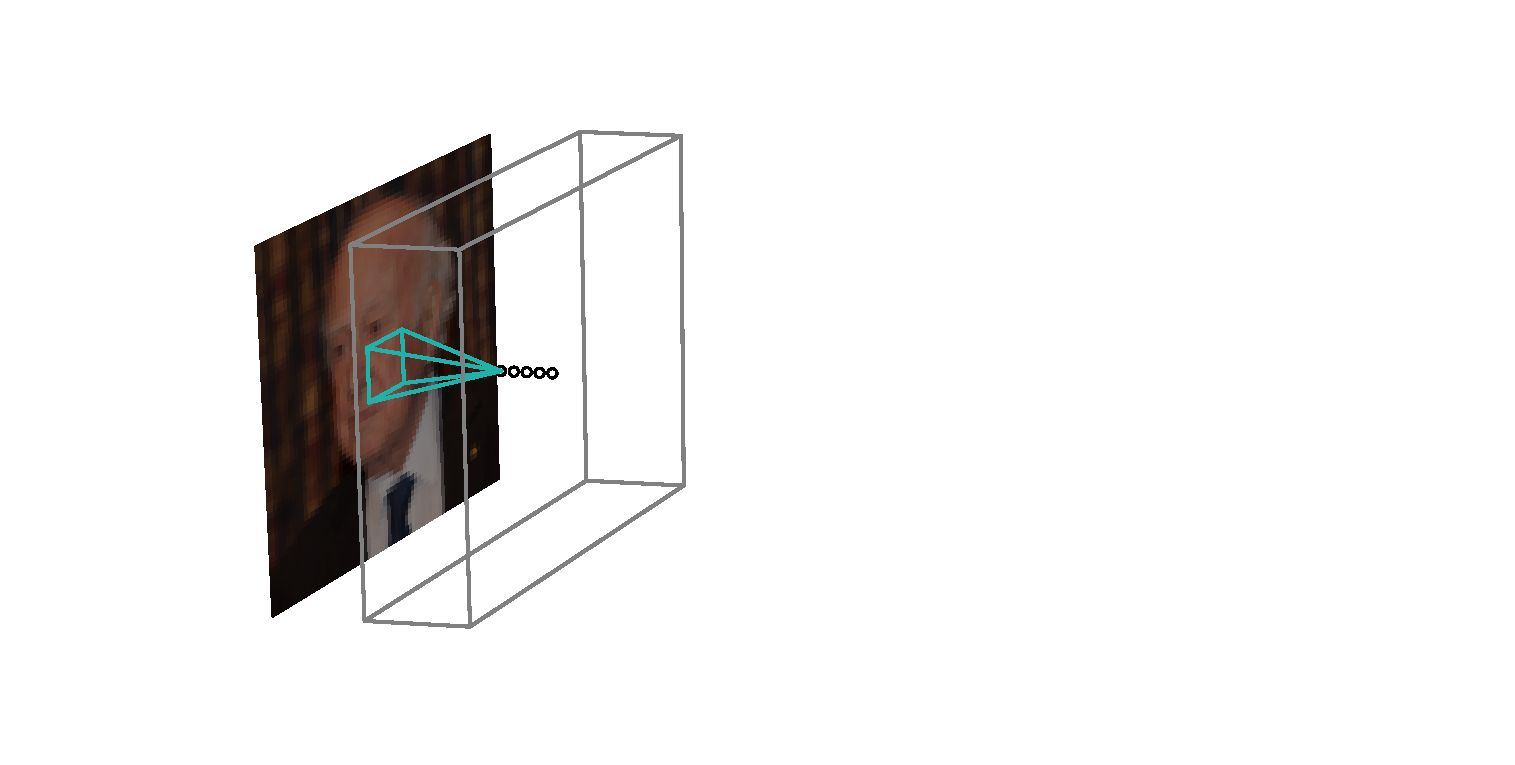
\includegraphics[width=0.32\textwidth]{figures/machine_learning/convolution_layer.pdf}
        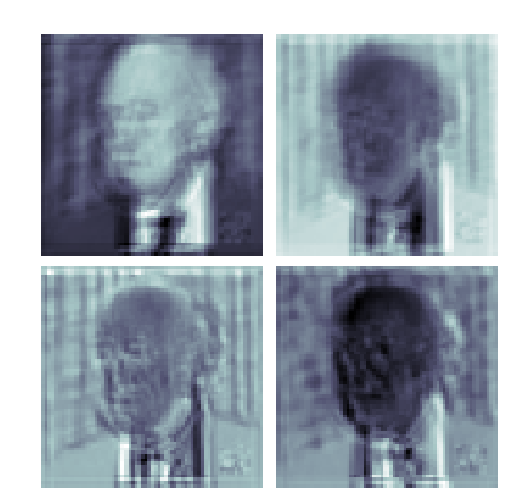
\includegraphics[width=0.32\textwidth]{figures/machine_learning/convolution_transforms.pdf}
    \end{center}
    \caption{Convolution layer: a single neuron connected and its connection to a $4\times{}4$ patch of input (left), an image patch and neurons in context with an input image \cite{Higgs_photo} (centre), and transformed versions of the input image with random filters (right).}
        \label{fig:machine_learning:convolution}
\end{figure}

This assumes that the filter is useful over the whole translational extent and leads to a much smaller quantity of parameters. As one has successive convolutions feed into each other low-level features are assembled into evermore sophisticated ones. Early layers will learn to detect edges, later ones combine these into shapes, and then later ones still into classes of objects such as cats or dogs. 


\subsubsection{Pooling Layers}
Pooling layers reduce the size of their input by mapping sections of neuron outputs to a single value, for example: a $2\times{}2$ patch, whilst keeping the depth the same.
This has the dual function of reducing model complexity and increasing the local field of view of later neurons. 
The two main types used are max pooling and average pooling (Figure \ref{fig:machine_learning:pooling}). 
\begin{figure}[h!]
    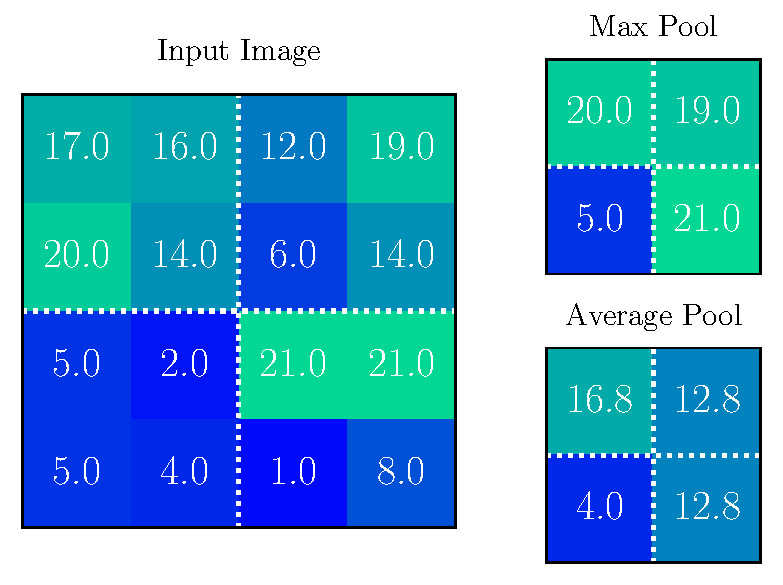
\includegraphics[width=0.45\textwidth]{figures/machine_learning/pooling.pdf}
    \caption{An example input to a pooling layer is shown on the left with two outputs on the right from max pooling (above) and average pooling (below).}
        \label{fig:machine_learning:pooling}
\end{figure}

Max pooling takes the maximal value in the region of interest and outputs this as the downsampled value. Max pooling leads faster trainings and to translation invariance of feature detection, but loses information and will cause the network to be less aware of the spatial arrangement of the features. 
Average pooling takes the average in the region of interest and does not throw away information, however it can be slower and does not have the same translation invariance properties. 


\subsubsection{Classic Architecture}
The classic example of a CNN consists of interleaved convolutional and pooling layers, at the end of these the feature map is flattened to a 1D array of neurons and then the rest of the network has the structure of an MLP (Figure \ref{fig:machine_learning:classic_CNN}). 
\begin{figure}[h!]
    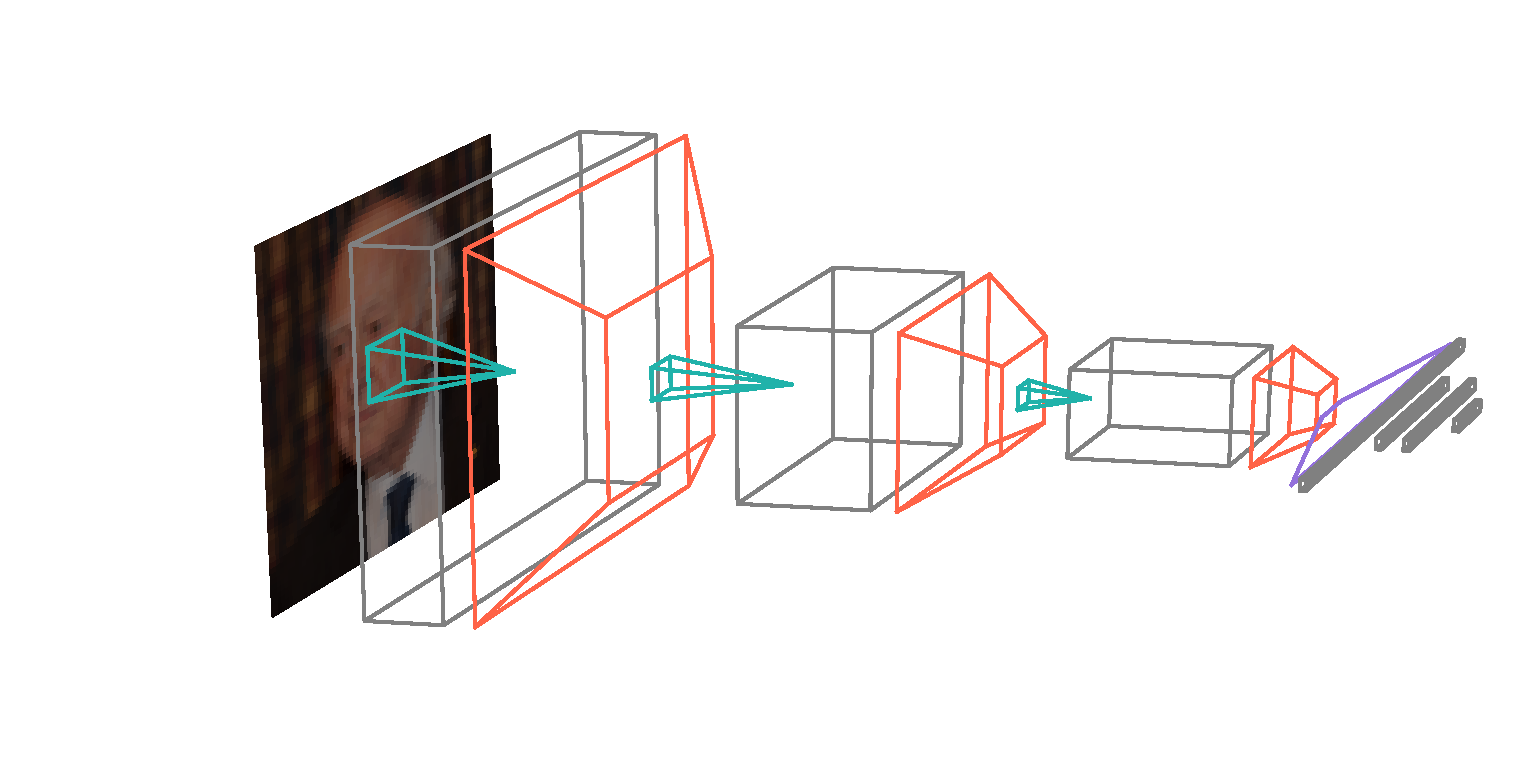
\includegraphics[width=0.85\textwidth]{figures/machine_learning/convnet_arch.pdf}
    \caption{A typical CNN architecture with three convolutional layers (grey) which contain neurons with a restricted FOV (green), pooling layers for downsampling (orange), a flattening of the final feature map (purple) and a set of fully-connected layers.}
        \label{fig:machine_learning:classic_CNN}
\end{figure}


\subsection{Dense Convolutional Neural Networks}
Dense convolutional neural networks \cite{DenseNet} are inspired by the bypass layers in models such as  ResNet, but here every layer is connected to every layer which comes after it. 
This gives superior information flow, encourages feature reuse, and allows the network to achieve high performance with fewer parameters. 

Dense CNNs have a similar general structure to ordinary CNNs: they are feedforward and make use of convolution and pooling, but their structure is much more complicated. 
Instead of interleaved convolution and pooling layers dense CNNs have dense blocks made of multiple composite layers of convolutions, these are interleaved with transition layers which play the role of pooling. After this the feature map is flattened and input to a MLP classifier structure as normal. 

\subsubsection{Composite Layers}
These layers are the basic unit which make up the dense blocks. They consist of (Figure \ref{fig:machine_learning:composite_layer}) a batch normalisation, a ReLU activation function, a $1\times{}1$ convolution which compresses the depth of the input volume, a second batch normalisation, a second ReLU activation and then an ordinary convolution which outputs a feature map of a set length $k$ called the growth rate. The $1\times{}1$ convolution is called a bottleneck and serves to reduce model complexity.
\begin{figure}[h!]
    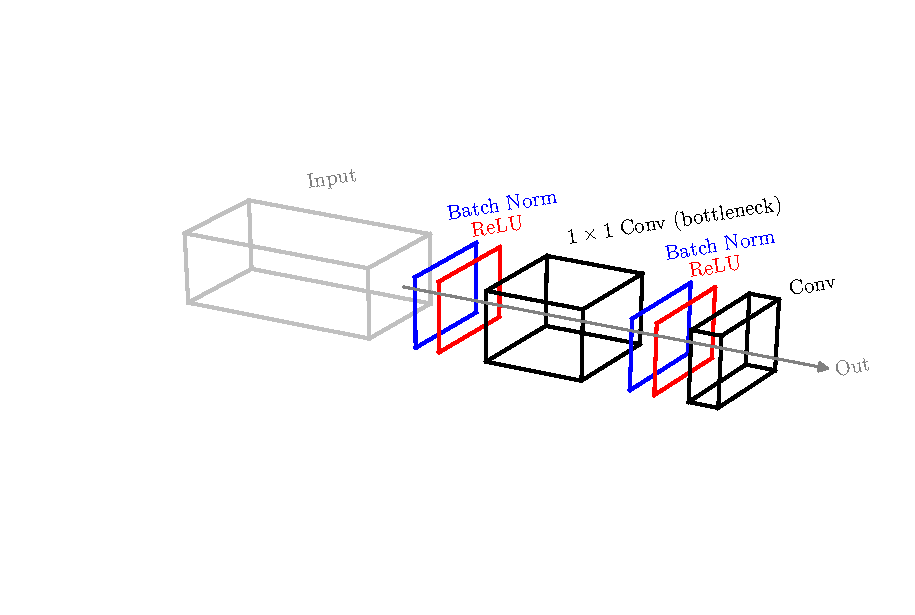
\includegraphics[width=0.75\textwidth]{figures/machine_learning/composite_layer.pdf}
    \caption{A composite layer}
        \label{fig:machine_learning:composite_layer}
\end{figure}


\subsubsection{Dense Blocks}
Dense blocks consist of $d$-many composite layers where there is direct connection from each layer to all those after it (Figure \ref{fig:machine_learning:dense_block}). 
In other word each layer receives all of the feature maps produced before it concatenated along the depth axis. 
\begin{figure}[h!]
    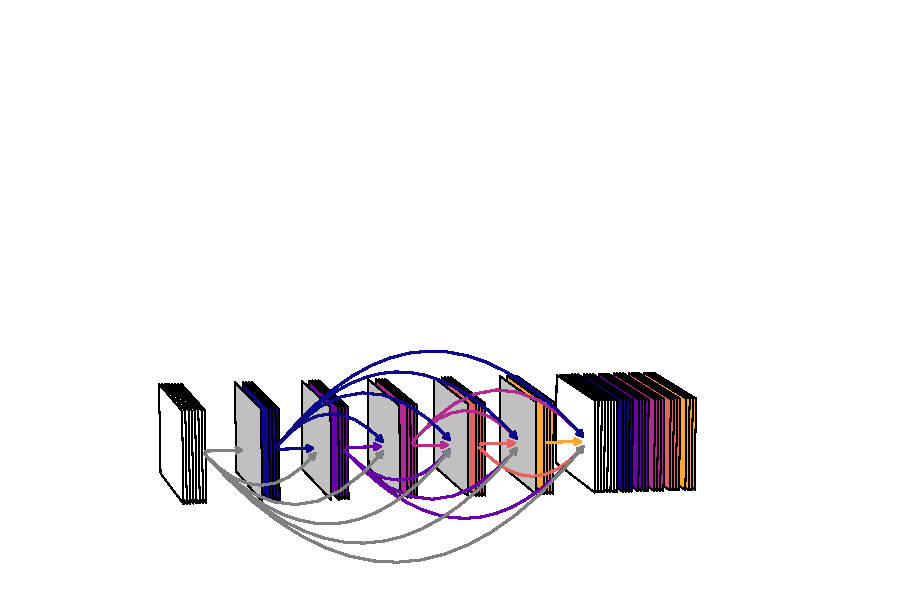
\includegraphics[width=0.75\textwidth]{figures/machine_learning/dense_block.pdf}
    \caption{A dense block with depth 5 and growth rate 4. Each composite layer is shown as a grey square and the output featuremap of the layer is shown by the coloured layered stack. Coloured arrows show the which layers each featuremap is input to.}
        \label{fig:machine_learning:dense_block}
\end{figure}
Each dense block has a number of hyperparameters. In the formulation used here they are the following: depth is the number of composite layers in the dense block, filter size is the width and height of the filter of the ordinary convolution in the composite layer, and the growth rate is the depth of the feature map from each composite layer.


\subsubsection{Transition Layers}
Transition layers are pooling layers with average pooling, but with batch normalisation applied to the input and a $1\times{}1$ convolution which compresses the input feature map before the pooling operation (Figure \ref{fig:machine_learning:transition_layer}). 
This compression of the feature map performs feature reduction where less useful features are removed. It will also reduce model complexity and overfitting. This reduction is controlled by another hyperparameter: the reduction factor. 
\begin{figure}[h!]
    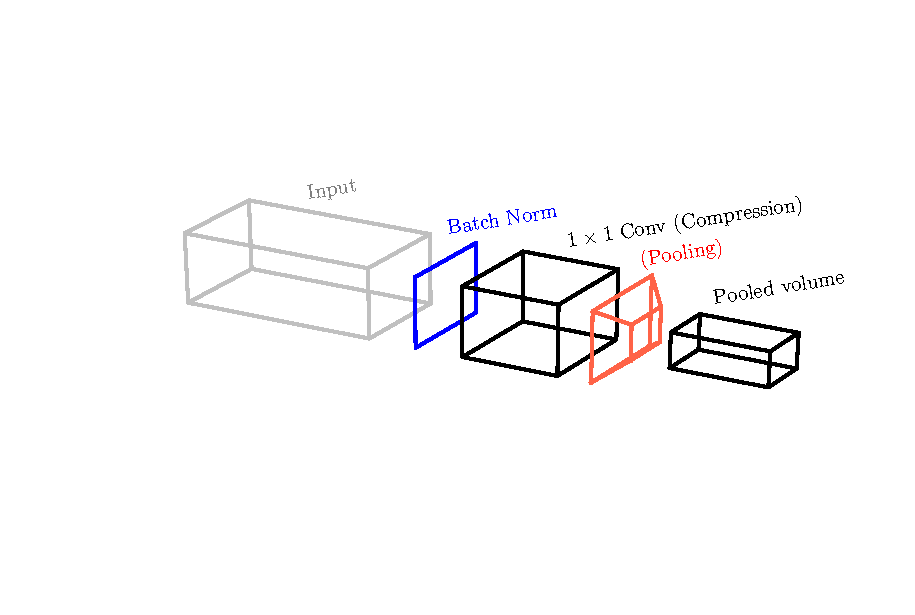
\includegraphics[width=0.75\textwidth]{figures/machine_learning/transition_layer.pdf}
    \caption{A transition layer with a reduction factor of 0.5.}
        \label{fig:machine_learning:transition_layer}
\end{figure}


